\begin{comment}
  http://www.visitusers.org/index.php?title=Running_client-server
\end{comment}

%% \begin{frame}{Distributed and remote visualization with VisIt}{}
%%   \begin{itemize}\setlength{\itemsep}{2mm}
%%   \item Working with fully remote VisIt
%%     \begin{itemize}\setlength{\itemsep}{0mm}
%%     \item ssh X-forwarding (X11 through ssh)
%%     \item remote VNC desktop
%%     \end{itemize}
%%   \item Client-server (remote VisIt server, local VisIt client)
%%   \item Parallel rendering
%%   \end{itemize}
%% \end{frame}

\begin{frame}{Visualizing remote data}
  So far we covered working with standalone VisIt on your desktop. If your dataset is on
  cluster.consortium.ca, you have many options to visualize it:\medskip
  \begin{enumerate}\setlength{\itemsep}{2mm}
  \item download data to your desktop and visualize it locally\\
    {\color{red} limited by dataset size and your desktop's CPU+GPU/memory}
  \item run VisIt remotely on a larger machine via X11 forwarding\\
    {\color{blue} your desktop $^{\underrightarrow{\rm ssh~-X}}$ larger machine running VisIt}
  \item run VisIt remotely on a larger machine {\bf via VNC}\\
    {\color{blue} your desktop $^{\underrightarrow{\rm VNC}}$ larger machine running VisIt}
    \begin{itemize}\setlength{\itemsep}{0mm}
    \item any node; preferably a GPU compute node
    \end{itemize}
  \item run VisIt in {\bf client-server mode}\\
    {\color{blue} VisIt viewer on your desktop $\rightleftharpoons$ VisIt on larger machine}
  \item run VisIt via a GUI-less batch script (interactively or scheduled)
  \end{enumerate}
  %% \medskip
  %% {\footnotesize
  %%   For remote options (2) - (5) the setup details vary across the consortia
  %%   \begin{itemize}\setlength{\itemsep}{0mm}
  %%   \item[-] render server can run with or without GPU rendering
  %%   \item[-] data/render servers can run on a single core, or across many cores/nodes with MPI
  %%   \item[-] for interactive GUI work on clusters it's best to schedule interactive jobs, as opposed to
  %%     running on the login nodes
  %%   \end{itemize}}
\end{frame}

\begin{frame}{X11 forwarding}
  \begin{itemize}\setlength{\itemsep}{3mm}
  \item Need a local X11 server (comes by default on Linux and Mac laptops) to which a remote application
    sends its window
  \item \texttt{ssh -X} lets you forward X11 graphics and mouse/keyboard interactions through ssh (encrypted!)
  \item Can forward through several consecutive connections, e.g.\\ laptop $^{\underrightarrow{\rm
      ssh~-X}}$ login node $^{\underrightarrow{\rm ssh~-X}}$ interactive development node
    \pause
  \item X11 forwarding is very chatty (lots of roundtrips!) and can be very slow on a high-latency
    network ... in general we don't recommend it
  \end{itemize}
\end{frame}

\begin{frame}{VNC (Virtual Network Computing)}
  \begin{itemize}\setlength{\itemsep}{3mm}
  \item Remote graphical desktop system
  \item Has gone to tremendous effort to optimize communication via data compression and caching
  \item Best to use VNC via an SSH tunnel and with a non-empty VNC password for higher security
    (virtually without a performance drop)
  \item Your remote collaborators can connect to the same VNC session with full keyboard/mouse control as long
    as they have the VNC password (different from your cluster password which should never be shared!)
  \item Setting it up connection is a little bit more involved, but well worth it
  \end{itemize}
\end{frame}

\begin{frame}{Remote VisIt via VNC on WestGrid (page 1 of 2)}{full details at \url{http://bit.ly/remotevnc}}
  \begin{enumerate}\setlength{\itemsep}{2mm}
  \item Install TurboVNC from \url{http://www.turbovnc.org} on your desktop
  \item Log in to parallel.westgrid.ca and run the command \texttt{vncpasswd}, at the prompt set a
    password for your VNC server (don't leave it empty) -- you'll use it in step 6
  \item {\bf\color{red} Submit an interactive job} to the cluster:\\
    {\footnotesize\texttt{qsub -q interactive -I -l nodes=1:ppn=1:gpus=1,walltime=1:00:00}}\\
    When the job starts, it'll return a prompt on the assigned compute node.
  \item On the compute node {\bf\color{red} start the vncserver}:\\
    \texttt{vncserver -geometry 1024x768}\\
    It'll produce something like {\it ``New 'X' desktop is cn0553:1''}, where the syntax is
    \texttt{nodeName:displayNumber}
  \end{enumerate}
\end{frame}

\begin{frame}{Remote VisIt via VNC on WestGrid (page 2 of 2)}{full details at \url{http://bit.ly/remotevnc}}
  \begin{enumerate}\setlength{\itemsep}{2mm}
  \item On your desktop {\bf\color{red} set up ssh forwarding} to the VNC port on the compute node:\\
    \texttt{ssh username@parallel.westgrid.ca -L xxxx:cn0553:yyyy}\\
    Here xxxx = 5901 is the local VNC port, and yyyy = 5900 (VNC's default) + \texttt{displayNumber}
    and is usually 5901 as well
  \item {\bf\color{red} Start TurboVNC vncviewer} on your desktop, enter \texttt{localhost:1} (that's
    xxxx-5900) and then enter the password from step 2 above
  \item A remote Gnome desktop will appear inside a VNC window on your desktop
  \item Inside this desktop start a terminal, use it to {\bf\color{red} start VisIt with a VirtualGL
    wrapper}\\
    {\footnotesize\texttt{vglrun /global/software/visit/visit271/bin/visit}}
  \end{enumerate}
\end{frame}

\begin{frame}{Client-server VisIt session}
  \vspace{-5mm}
  \begin{columns}
    \begin{column}{7.25cm}
      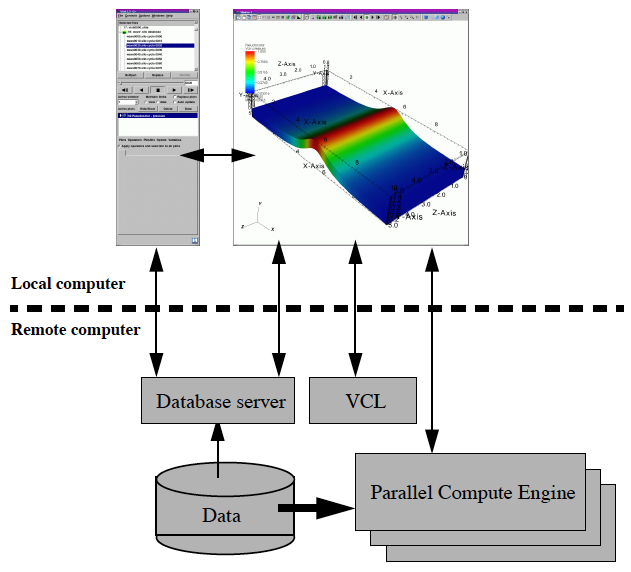
\includegraphics[width=\columnwidth]{figs/visit-guis/VisIt_arch}
    \end{column}
    \begin{column}{5.00cm}
      \begin{itemize}\setlength{\itemsep}{3mm}
      \item{\footnotesize Your local VisIt will start remote VCL (VisIt Component Launcher) responsible
        for launching other remote VisIt components}
      \item{\footnotesize Require:}
        \begin{enumerate}\setlength{\itemsep}{0mm}
        \item{\scriptsize properly configured VisIt on the HPC system}
        \item{\scriptsize a host profile (configured by HPC support staff) to tell your local VisIt
          how to connect and how to launch VCL on the HPC system (could be a queued job)}
        \end{enumerate}
      \end{itemize}
    \end{column}
  \end{columns}
\end{frame}


%% abc
%% parallel
%% qsub -q interactive -I -l nodes=1:ppn=4:gpus=1,walltime=0:30:00
%% visit -l mpirun -np 4     # will it print the port #?
%% need to recompile the MPI version?





%% laptop
%% Options \ra Host profiles and Configuratin Setup
%% select None (use VisIt's standard defaults)
%% Options \ra Host profiles
%% cn0553





%% The specific error was: "<The reason for the exception was not described>"

%% It is possible that SSH was unable to launch VisIt on parallel.westgrid.ca. If you want to verify this, run "visit -debug 5" and then check to see if any vcl, mdserver, or engine log files are present on parallel.westgrid.ca in your home directory. If no log files were created then SSH was probably not able to launch VisIt components on parallel.westgrid.ca. In that case, check that you can SSH to parallel.westgrid.ca and check your local VisIt installation's Host profiles to make sure the path to VisIt on parallel.westgrid.ca is specified. Alternatively, you set the PATH environment variable on parallel.westgrid.ca so it contains the path to the program "visit".

%% If there were no debug logs to be found on parallel.westgrid.ca and your local computer runs a newer version of Linux then quit VisIt and try running "visit -nopty -debug 5". The "-nopty" option tells VisIt not to allocate a pseudoterminal in which to run SSH. When you run with the "-nopty" option, VisIt's password window will not be used. Instead, look for an SSH prompt in the terminal window where you ran VisIt. You should be able to enter your password at that prompt. If successful, SSH should continue trying to launch VisIt on parallel.westgrid.ca. If VisIt still cannot connect after SSH launches VisIt's remote components, check for debug logs on parallel.westgrid.ca to see if VisIt was at least able to launch there.

%% "vglrun": If you do not know what "vglrun" is, you can ignore this paragraph.  If there were no debug logs to be found on parallel.westgrid.ca and you are using vglrun, then vglrun may be causing VisIt to fail. Some versions of vglrun cause the ssh program to fail.  If you are running VisIt in conjunction with vglrun, this may be causing your failure.  (You can test this by running "vglrun ssh" and seeing if it cores.)

%% If you found debug log files on parallel.westgrid.ca but VisIt still can't connect then it's possible that parallel.westgrid.ca cannot connect to your local computer. Some desktop computers do not provide a valid network name when VisIt asks for one. If you suspect that this could be the cause of the launch failure, try using "Parse from SSH_CLIENT" in your host profile for host parallel.westgrid.ca. If that does not work and if you are using VPN then you should try manually setting the local host name VisIt will use when telling its remote components to connect back to your local computer. Open the Host profiles window and go to the Advanced options tab. Click the "Specify manually" radio button and type in the IP address of your VPN session into the adjacent text field before you try connecting again.

%% If changing the above settings still does not allow you to connect then you may have a local firewall blocking ports 5600-5609, which are the ports that VisIt uses to listen for incoming connections (when they are expected) from remote VisIt components. If you've tried the previous suggestions and none of them worked then you may have a firewall denying VisIt access to local computer. Try turning the firewall off or allowing ports 5600-5609 and run VisIt again. If you do not know how to enable ports for your firewall or if you do not have the required privileges, contact your system administrator.

%% If none of these suggestions allow you to successfully connect to parallel.westgrid.ca then contact visit-users@ornl.gov and provide information about how you are trying to connect. Be sure to include the VisIt version and platform on which you are running.
